\begin{frame}{Survival Analysis}
\begin{block}{Survival Analysis}
Survival analysis is a field of statistics concerned with analyzing time to 
event data, often in the face of censoring or truncation.
\end{block}
Example:
\begin{itemize}
 \item The survival of patients after brain mets from breast cancer
 \item Censoring/Truncation:
 \begin{itemize}
  \item study ending and no death 
  \item subject dies before study starts
  \item subject moves away and can't contact them 
 \item exact death time only known in an interval
 \end{itemize}

\end{itemize}
\end{frame}

\begin{frame}{Kaplan-Meier Estimator}
\begin{itemize}
 \item The survival function $S(t)=P(T>t)=\int_{t}^{\infty}f(u)du$ is estimated by the 
 nonparametric Kaplan-Meier Estimator
 $$\hat{S}(t)=\prod_{t_i<t}\frac{n_i -d_i}{n_i}$$
\item $n_i$ is the number of subject in the risk set at time $t_i$
\item $d_i$ is the number of deaths at time $t_i$
\end{itemize}
 \begin{figure}[h!]
  \centering
    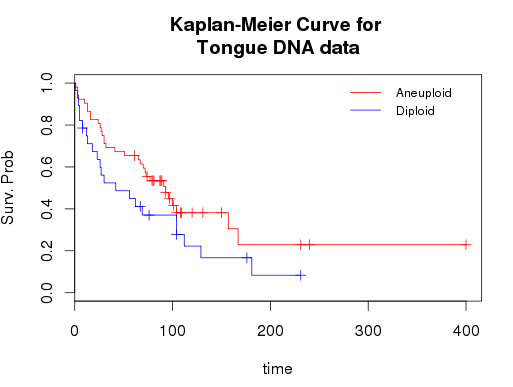
\includegraphics[width=0.38\textwidth]{km_example.png}
  \caption{Tongue Cancer date from \cite{Klein1984}}
\label{fig:KMcurve}
\end{figure}
\note{
 risk set at time t; the set of individuals alive and uncensored just before time t.
We use death and survival because easy to say, but it really means event or not}
\end{frame}

\begin{frame}{Log rank test}
$H_0$: No difference between the survival curves of the two populations

$$\frac{\sum_{j=1}^{J}(O_{1j}-E_{1j})}{\sqrt{\sum_{j=1}^{j}V_{j}}}\sim N(0,1)$$
\begin{itemize}
 \item $N_j=N_{1j}+N_{2j}$ is the number at risk at time j (composed from deaths in each group)
 \item $O_j=O_{1j}+O_{2j}$ is the observed number of deaths at time j (composed from the observed deaths in each group)
 \item $E_{1j}=\frac{O_jN_{1j}}{N_j}$
 \item $V_j=\frac{O_j(N_{1j}/N_j)(1-N_{1j}/N_j)(N_{j}-O_{j})}{N_j -1}$
 \end{itemize}
%\note[itemize]{ mention weights?
%}
\end{frame}


\begin{frame}{Hazard Function}
%might want to use the underbraces
%$\underbrace{h_{0}(t)}_{\textrm{time}}*\underbrace{exp(\sum_{k=1}^{p}\beta_{k}Z_{k})}_{\textrm{covariates}}$
\begin{itemize}
 \item Hazard is the instantaneous rate of event given that you have survived until time t, given 
 by $$h(t)=\lim_{\Delta t \rightarrow 0+}\frac{P[t\leq T<t+\Delta t|T\geq t]}{\Delta t}$$
\end{itemize}
 \begin{figure}[h!]
  \centering
    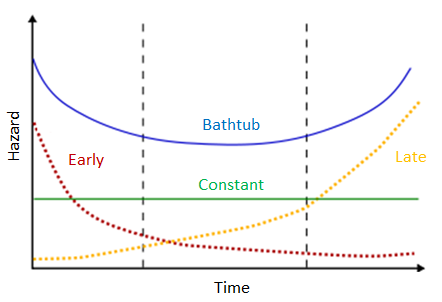
\includegraphics[width=0.55\textwidth]{hazard.png}
  \caption{A few different hazard function shapes \cite{wikihazard}}
\label{fig:hazard}
\end{figure}
\end{frame}

\begin{frame}{Cox Regression}
\begin{itemize}
   \item Cox regression models hazard by 
   
   %$$h(t|Z)=h_{0}(t)\exp(\sum_{k=1}^{p}\beta_{k}Z_{k})$$
   $$h(t|Z)=\underbrace{h_{0}(t)}_{\textrm{time}}*\underbrace{exp(\sum_{k=1}^{p}\beta_{k}Z_{k})}_{\textrm{covariates}}$$

   \item Where $h_{0}(t)$ is the baseline hazard
   \item $Z_k$ is the $k^{th}$ covariate
   \item $\beta_k$'s are found by maximizing the partial likelihood function
\item The covariates act to multiply the hazard function.
\end{itemize}

\end{frame}
